\section {GIF}
\subsection {Pourquoi le GIF?}
Le format GIF permet de stocker plusieurs images dans un fichier. Ceci permet de créer des diaporamas, voire des animations si les images sont affichées à un rythme suffisamment soutenu. Chaque image d'une animation peut avoir sa propre palette.
Le GIF est un format très utilisé, particulièrement sur les réseaux sociaux. Ce projet peut donc intéressé pas mal de gens. ////
La structure du format GIF est connue et disponible en ligne. En voici un schéma : 
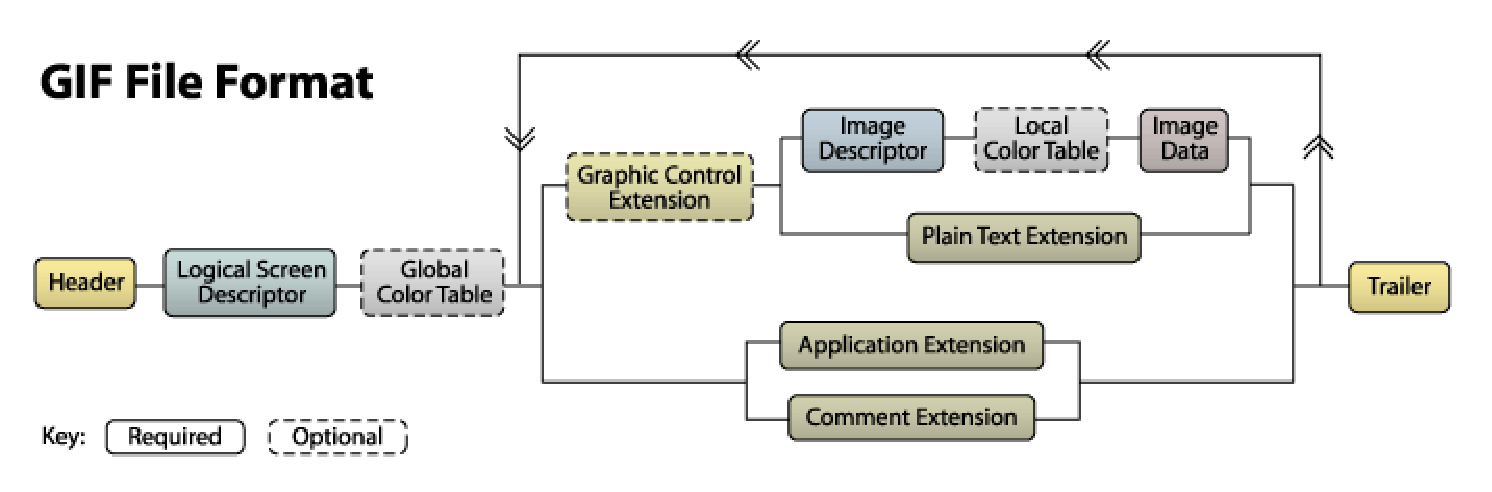
\includegraphics[width=8cm]{gif_structure.eps}
\subsection {Application du LSB}
Nous avons choisi de cacher des informations dans les couleurs qui se trouvent dans les Local Color Table. Cette section facultative peut revenir devant chaque bloc image data. Si cette section n'existe pas, nous la rajoutons.\\\\
Il est possible de calculer la taille maximale du message cachée à l'avance, en comptant le nombre de bloc image data et en le multipliant par le nombre de byte dans la Global Color Table.
\subsection {Avancement}
\subsection {Guide pratique}
\newpage
%
%
%
%
\section {exemples latex}
Vous découpez votre travail en chapitre (section), en sous-chapitre (subsection) et en sous-sous-chapitre (subsubsection)
Il suffit de taper le texte au kilomètre. \emph{Il est possible d'insister} sur un passage.
Vous appelez la commande :
\lstset{frame=trBL}
\begin{lstlisting}
aspell -t - -encoding='iso8859-15' -c VotreFichier.tex
\end{lstlisting}
\subsubsection {Une énumération}
Si vous devez utiliser des puces :
\begin{itemize}
\item point 1
\item point 2
\end{itemize}
Si vous devez énumérer :
\begin{enumerate}
\item point 1
\item point 2
\end{enumerate}
Vous pouvez mélanger à autant de niveaux que vous le souhaitez.
\subsubsection{Un tableau}
\begin{tabular}{|l|l||c||r|} %left ou r ou c ou p[dimension]
\hline
Jour & Heures & Local & Cours \\
\hline
Mardi    &  3..4  & 503 & Système\\
Mardi    &  5..8  & 503 & Sécurité\\
\hline
Mercredi  &  1..2  &  201 & Assembleur\\
Mercredi  &  3..4  &  003 & Labo assembleur\\
\hline
\end{tabular}
\subsubsection {Intégrer une source}
Pour énumérer une source, vous pouvez préciser ce que vous souhaitez avec lstset. 
\lstset{language={},frame=trBL}
\begin{lstlisting}
MOV EAX,10 ; place 10 dans le registre EAX
ADD EAX,20 ; ajoute 20 au contenu de EAX
\end{lstlisting}
\subsubsection {Intégrer un graphique}
Vous pouvez intégrer un graphique mais il faut qu'il soit en format eps.\\
Vous pouvez dessiner avec l'outil oodraw qui permet d'exporter votre dessin dans ce format eps.\\
Vous pouvez transformer un jpeg en eps avec l'outil sam2p ou convert qui se trouve dans le package ImageMagick\\
%\includegraphics[width=8cm]{Dessin.eps}
\subsubsection {Mode mathématique}
C'est un des points forts de latex qui permet d'écrire des formules mais aussi des caractères spéciaux tels que :
$2^{32} \approx 10^{9}$ car $\log{_{10}}{2} \approx 0.3$ et $32*0.3 \approx 9$.
\subsubsection {Quelques trucs faciles}
\begin{itemize}
\item \verb+\\+ permet de passer à la ligne suivante.
\item \verb+\\[2cm]+ permet de passer à la ligne suivante + une tabulation verticale de 2cm. Sont autorisés mm, cm et pts.
\item \verb+\newpage+ permet de forcer un passage à la page suivante.
\end{itemize}
\subsubsection {Compiler le texte}
Un script permet d'automatiser cette compilation:
\begin{lstlisting}
#! /bin/sh
FN=Mrapport # Le nom du document.
latex $FN.tex
latex $FN.tex # 2 passages pour la TOC
rm $FN.aux $FN.log $FN.out
dvips $FN.dvi -o $FN.ps
rm $FN.dvi
gv $FN.ps # pour visualiser et imprimer
\end{lstlisting}
%-----------------------------------------------------------------------------------
\subsection{Conclusions}
Ce travail montre, qu'en quelques minutes, on peut déjà fournir un travail présenté de façon professionnelle, lisible par tous et dans un format standard.
Pour ne pas avoir de soucis, les commandes à utiliser pour obtenir un document postcript sont latex et dvips, il ne faut jamais utiliser pdflatex. 

Ce document peut être encore complété avec d'autres exemples qui seraient utiles. Ces nouveaux exemples pourraient être intégrés dans le premier ou un deuxième chapitre. Ceci, sans oublier qu'il s'agit d'un document utile pour commencer très rapidement à écrire en latex et non un mode d'emploi complet de latex qui serait obligatoirement très volumineux.
%-----------------------------------------------------------------------------------
\subsection{Références}
\begin{itemize}
\item http://www.grappa.univ-lille3.fr/FAQ-LaTeX/ 
\item http://tex.loria.fr/
\item http://tex.loria.fr/english/packages.html
\end{itemize}
%-----------------------------------------------------------------------------------
\subsection{Annexes }
Vous trouvez dans le casier, un répertoire LATEX contenant :
\begin{itemize}
\item Mrapport.tex : le document latex maître
\item LatexSimple.tex : ce document latex
\item dessin.odg et dessin.eps : le dessin intégré dans le texte
\item go : un script qui permet de compiler rapport.tex, sans argument.
\end{itemize}
%-----------------------------------------------------------------------------------
